\documentclass[./main.tex]{subfiles}

\begin{document}

\subsection{Telegraf}

Je Open source server agent vytvorený v programovacom jazyku GO na zbierania metrík z udalostí z databáz, senzorov a systémov. Podporuje viac ako 200 pluginov pre rôzne používané technológie. Telegraf je schopný spárovať dáta z formátov: InfluxDB Line Protocol, JSON, Graphite, Value, Nagios, a Collectd. Telegraf plugin podporuje procesy, ale nie je treba zmeniť ich štruktúru.
\begin{figure}[h!]
    \centering
    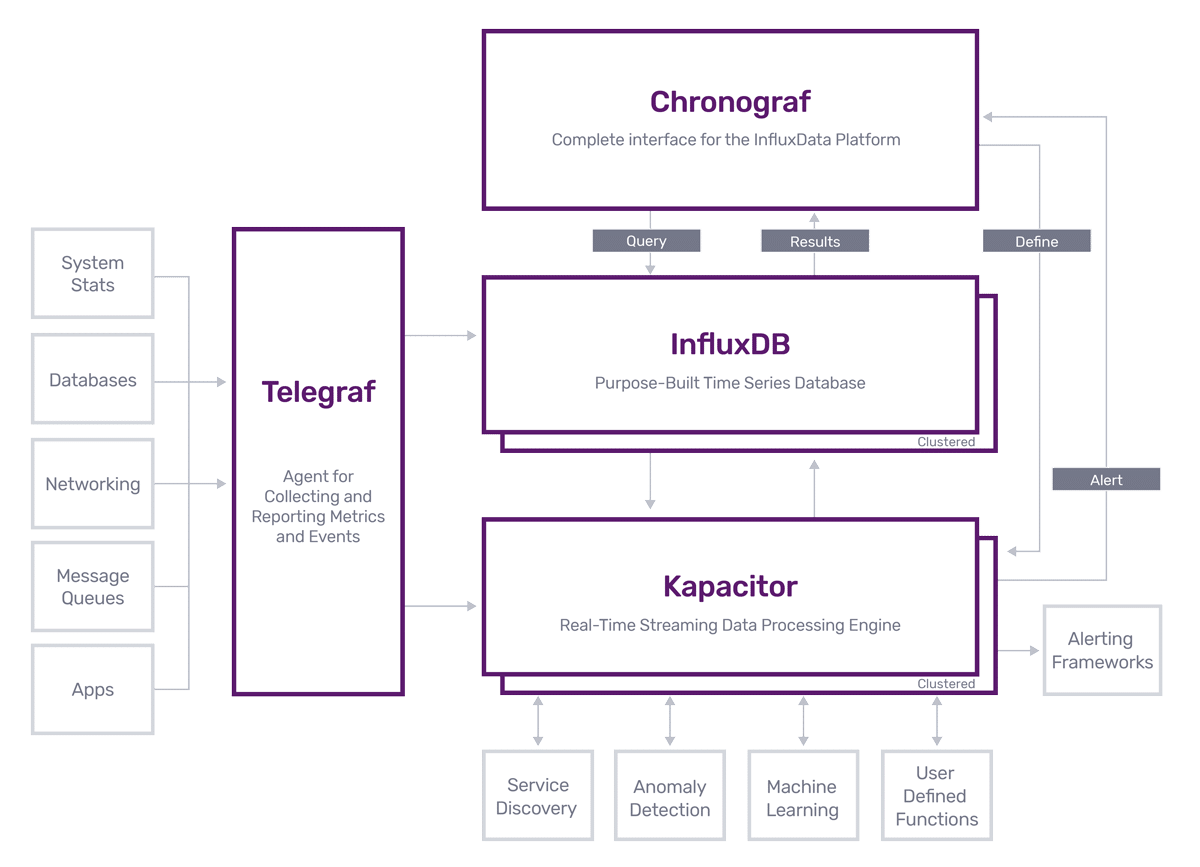
\includegraphics[width=0.9\textwidth]{images/telegraf.png}
    \caption{Použitie InfluxDB a Telegraf - diagram\cite{telegraf}}
    \label{fig:telegraf}
\end{figure}


\end{document}